% Provenance (never printed): see sources/outline_sources.md (Year 3:
% concordia and discordia; 40Ar/39Ar step heating; Sm-Nd model ages;
% cosmogenic nuclides; fission tracks and (U-Th)/He). Brief:
% sources/book5/BRIEFS.md, ch. 13. Curves from figdata/bachelor-3/
% concordia.py, arar_spectrum.py, model_ages.py, cosmogenic.py. Exercise and
% problem values in the Book 5 scratch calculator calc/ch13.py. The zircons,
% the biotite spectrum, the Nd sample and the helium ages of the Varden
% granite are invented, consistent with the Year 1 volume's granite of 310 Ma.
\chapter{Geocronología avanzada}\label{ch:b3:advanced-geochronology}

Un cristal de circón de una décima de milímetro de largo ha mantenido en marcha dos relojes
desde que cristalizó su granito: el uranio-238 que se desintegra en plomo-206 y
el uranio-235 que se desintegra en plomo-207. Cuando los dos relojes coinciden, la edad
es indudable. Cuando discrepan, la propia discrepancia puede datarse: el
cristal perdió parte de su plomo en un evento posterior, y los dos relojes, leídos
en conjunto, dan la edad del granito y la del evento. Este capítulo
lee varios relojes a la vez, en uranio y plomo, en argón, en neodimio, en
trazas de fisión y helio, y en los átomos raros producidos por los rayos cósmicos, y
indica hasta qué punto cabe fiarse de cada edad.

\begin{recall}
La desintegración radiactiva, la ecuación de la edad, la isócrona y su razón inicial, la
recta de mínimos cuadrados, la desintegración ramificada, la edad potasio--argón, la
temperatura de cierre y la edad de enfriamiento están en el volumen de primer año, en su capítulo sobre
datación radiométrica; la fórmula de erosión estacionaria de los \omterm{def:b3:advanced-geochronology:cosmogenic}{nucleidos cosmogénicos} está en
su capítulo sobre erosión y transporte. El reservorio condrítico uniforme, la
notación épsilon y el manto empobrecido están en el volumen de segundo año, en su
capítulo sobre geoquímica isotópica; la ionización térmica y la espectrometría de masas
multicolector, en su capítulo sobre métodos de campo y de laboratorio. La \omterm{def:b3:orogenic-wedges:thermochronology}{termocronología} y
la \omterm{def:b3:orogenic-wedges:age-elevation}{relación edad--altitud} están en el \cref{ch:b3:orogenic-wedges}.
\end{recall}

\section{Uranio, plomo y la concordia}\label{sec:b3:advanced-geochronology:upb}

El uranio tiene dos isótopos de vida larga. El uranio-238 se desintegra a través de una cadena de
hijas de vida corta hasta el plomo-206, con $\lambda_{238} =
\qty{1.55125e-10}{yr^{-1}}$; el uranio-235 se desintegra en plomo-207 con $\lambda_{235}
= \qty{9.8485e-10}{yr^{-1}}$, seis veces más rápido. Su razón actual es
$^{235}\mathrm{U}/^{238}\mathrm{U} = 0.0072567$, o bien $^{238}\mathrm{U}/^{235}\mathrm{U}
= 137.8$, la misma en toda roca terrestre. El circón, $\mathrm{ZrSiO_4}$, incorpora
mucho uranio y casi nada de plomo al crecer, y resiste la meteorización
y sobrevive al metamorfismo: casi todo su plomo es radiogénico.
% ledger: amherst:constants, tulane:upb-zircon

Se definen $x = {}^{207}\mathrm{Pb}^*/{}^{235}\mathrm{U}$ e $y =
{}^{206}\mathrm{Pb}^*/{}^{238}\mathrm{U}$ como razones actuales del plomo radiogénico
respecto a su progenitor. Cada una da una edad, $t_{206} = \ln(1 + y)/\lambda_{238}$
y $t_{207} = \ln(1 + x)/\lambda_{235}$.

\begin{definition}[Concordia, discordia, intersecciones, diagrama de Tera--Wasserburg]
\label{def:b3:advanced-geochronology:concordia}
La \emph{concordia}\index{concordia} es la curva del plano $(x, y)$ en la que
las dos edades uranio--plomo son iguales. Una \emph{discordia}\index{discordia}
es una recta a lo largo de la cual se alinean los análisis discordantes de una misma población de
cristales; sus intersecciones con la concordia son la
\emph{intersección superior}\index{intersección superior} (la más antigua) y la
\emph{intersección inferior}\index{intersección inferior} (la más joven). El
\emph{diagrama de Tera--Wasserburg}\index{diagrama de Tera--Wasserburg} representa
$X = {}^{238}\mathrm{U}/{}^{206}\mathrm{Pb}^*$ frente a $Y =
{}^{207}\mathrm{Pb}^*/{}^{206}\mathrm{Pb}^*$.
\end{definition}

\begin{theorem}[La concordia]\label{thm:b3:advanced-geochronology:concordia}
Un cristal que ha permanecido cerrado al uranio y al plomo desde que se formó, hace
un tiempo $t$, se sitúa en
\[
C(t) = \bigl(e^{\lambda_{235}t} - 1,\; e^{\lambda_{238}t} - 1\bigr).
\]
A medida que $t$ crece, la curva sube cada vez más despacio frente a $x$: su pendiente,
$\mathrm dy/\mathrm dx = (\lambda_{238}/\lambda_{235})\,e^{(\lambda_{238} -
\lambda_{235})t}$, decrece desde $\lambda_{238}/\lambda_{235} = 0.1575$ en el
origen, de modo que la \omterm{def:b3:advanced-geochronology:concordia}{concordia} es cóncava hacia el eje $x$.
\end{theorem}

\begin{proof}
Para cada progenitor, el número de hijas radiogénicas por átomo progenitor que queda es
$e^{\lambda t} - 1$, la ecuación de la edad del volumen de primer año. Derivando
ambas coordenadas respecto de $t$ y dividiendo se obtiene la pendiente; dado que
$\lambda_{235} > \lambda_{238}$, decrece con $t$.
\end{proof}

El plomo es un ion grande que encaja mal en la red del circón. En las zonas de un
cristal dañadas por su propia radiactividad, puede perderse en un evento posterior de
calentamiento o circulación de fluidos.
% ledger: tulane:upb-zircon

\begin{theorem}[La pérdida episódica de plomo da una cuerda]\label{thm:b3:advanced-geochronology:discordia}
Un cristal que se formó hace un tiempo $t_1$ y que perdió, hace un tiempo $t_2$, una fracción $f$
de su plomo radiogénico, y que por lo demás permaneció cerrado, se sitúa hoy en
\[
(1 - f)\,C(t_1) + f\,C(t_2),
\]
sobre la cuerda que une los puntos $t_1$ y $t_2$ de la \omterm{def:b3:advanced-geochronology:concordia}{concordia}. Los cristales que
perdieron fracciones distintas se alinean sobre esa cuerda, una \omterm{def:b3:advanced-geochronology:concordia}{discordia} cuya
\omterm{def:b3:advanced-geochronology:concordia}{intersección superior} es $t_1$ y la inferior es $t_2$.
\end{theorem}

\begin{proof}
Se considera un sistema de desintegración, con constante $\lambda$, y se cuenta por átomo de progenitor
presente hoy. Hace un tiempo $t_2$ había $e^{\lambda t_2}$ átomos progenitores, y
hijas radiogénicas $e^{\lambda t_2}(e^{\lambda(t_1 - t_2)} - 1) =
e^{\lambda t_1} - e^{\lambda t_2}$. El evento dejó $(1 - f)(e^{\lambda t_1} -
e^{\lambda t_2})$; desde entonces el progenitor generó $e^{\lambda t_2} - 1$ más. La
suma es $(1 - f)(e^{\lambda t_1} - 1) + f(e^{\lambda t_2} - 1)$. Los dos isótopos
de plomo se comportan igual químicamente, así que $f$ es la misma para ambos, y las dos
coordenadas se combinan en el punto enunciado.
\end{proof}

\begin{omfigure}
\begin{tikzpicture}
\begin{groupplot}[group style={group size=2 by 1, horizontal sep=1.7cm},
  omrecord, width=0.47\linewidth, height=0.42\linewidth, title style={font=\small},
  tick label style={font=\scriptsize}, label style={font=\small}]
\nextgroupplot[title={(a) diagrama de la concordia},
  xlabel={$^{207}\mathrm{Pb}^*/^{235}\mathrm{U}$}, ylabel={$^{206}\mathrm{Pb}^*/^{238}\mathrm{U}$},
  xmin=0.04, xmax=0.44, ymin=0.006, ymax=0.06,
  xtick={0.1,0.2,0.3,0.4}, xticklabels={0.1,0.2,0.3,0.4},
  ytick={0.01,0.02,0.03,0.04,0.05}, yticklabels={0.01,0.02,0.03,0.04,0.05},
  scaled ticks=false]
% computed in figdata/bachelor-3/concordia.py
\addplot[black, thick] table[x=xw, y=yw] {figdata/out/bachelor-3-concordia-curve.dat};
\addplot[black, only marks, mark=*, mark size=1.4pt, nodes near coords={\scriptsize\pgfmathprintnumber[fixed, precision=0]{\pgfplotspointmeta}},
  point meta=explicit, nodes near coords align={anchor=south east},
  restrict expr to domain={\thisrow{t}}{100:350}]
  table[x=xw, y=yw, meta=t] {figdata/out/bachelor-3-concordia-ticks.dat};
\addplot[omDef, thick, densely dashed] table[x=x, y=y] {figdata/out/bachelor-3-concordia-line.dat};
\addplot[red!70!black, only marks, mark=diamond*, mark size=2pt] table[x=x, y=y] {figdata/out/bachelor-3-concordia-zircons.dat};
\nextgroupplot[title={(b) diagrama de Tera--Wasserburg},
  xlabel={$^{238}\mathrm{U}/^{206}\mathrm{Pb}^*$}, ylabel={$^{207}\mathrm{Pb}^*/^{206}\mathrm{Pb}^*$},
  xmin=15, xmax=75, ymin=0.0465, ymax=0.0535,
  ytick={0.047,0.049,0.051,0.053}, yticklabels={0.047,0.049,0.051,0.053},
  scaled ticks=false]
\addplot[black, thick] table[x=xtw, y=ytw] {figdata/out/bachelor-3-concordia-curve.dat};
\addplot[black, only marks, mark=*, mark size=1.4pt, nodes near coords={\scriptsize\pgfmathprintnumber[fixed, precision=0]{\pgfplotspointmeta}},
  point meta=explicit, nodes near coords align={anchor=north east},
  restrict expr to domain={\thisrow{t}}{100:250}]
  table[x=xtw, y=ytw, meta=t] {figdata/out/bachelor-3-concordia-ticks.dat};
\addplot[omDef, thick, densely dashed] table[x=xtw, y=ytw] {figdata/out/bachelor-3-concordia-twline.dat};
\addplot[red!70!black, only marks, mark=diamond*, mark size=2pt] table[x=xtw, y=ytw] {figdata/out/bachelor-3-concordia-zircons.dat};
\end{groupplot}
\end{tikzpicture}

\par\smallskip{\small (a) La \omterm{def:b3:advanced-geochronology:concordia}{concordia}, con sus edades en millones de años,
y cinco circones discordantes inventados de un mismo granito (en rojo; sus elipses de error
son más pequeñas que los símbolos), alineados sobre una \omterm{def:b3:advanced-geochronology:concordia}{discordia} (discontinua) que
corta a la \omterm{def:b3:advanced-geochronology:concordia}{concordia} cerca de 311 y \qty{100}{\Ma}. (b) Los mismos circones y la misma recta
en el \omterm{def:b3:advanced-geochronology:concordia}{diagrama de Tera--Wasserburg}, donde una \omterm{def:b3:advanced-geochronology:concordia}{discordia} sigue siendo una
recta.}\label{fig:b3:advanced-geochronology:concordia}
\end{omfigure}
% ledger: amherst:constants

Las intersecciones se hallan donde $a + b\,x(t) = y(t)$, una ecuación en $t$ que
se resuelve por el método de Newton: con $g(t) = e^{\lambda_{238}t} - 1 - a -
b(e^{\lambda_{235}t} - 1)$ y $g'(t) = \lambda_{238}e^{\lambda_{238}t} -
b\lambda_{235}e^{\lambda_{235}t}$, iterando $t \leftarrow t - g/g'$ a partir de una estimación
cercana a cada intersección. Tres propiedades del resultado importan en la práctica.
En primer lugar, la \omterm{def:b3:advanced-geochronology:concordia}{intersección superior} solo es precisa si la \omterm{def:b3:advanced-geochronology:concordia}{discordia} corta a la
\omterm{def:b3:advanced-geochronology:concordia}{concordia} con un ángulo grande. Una \omterm{def:b3:advanced-geochronology:concordia}{discordia} joven, como en la figura anterior, discurre
casi a lo largo de la \omterm{def:b3:advanced-geochronology:concordia}{concordia}, y un pequeño cambio en su pendiente desplaza la
intersección mucho. En segundo lugar, si la pérdida de plomo es reciente, $t_2 = 0$, la \omterm{def:b3:advanced-geochronology:concordia}{discordia}
pasa por el origen, y todos los cristales tienen la misma
razón $^{207}\mathrm{Pb}^*/^{206}\mathrm{Pb}^*$,
\[
\frac{^{207}\mathrm{Pb}^*}{^{206}\mathrm{Pb}^*} = \frac{1}{137.8}\,
\frac{e^{\lambda_{235}t_1} - 1}{e^{\lambda_{238}t_1} - 1},
\]
lo que da $t_1$ sin necesidad del uranio: la edad plomo--plomo. En tercer lugar, una recta en el
diagrama de la \omterm{def:b3:advanced-geochronology:concordia}{concordia}, $x = (y - a)/b$, se convierte en las coordenadas de Tera--Wasserburg
$Y = (1 - aX)/(137.8\,b)$, de nuevo una recta. El \omterm{def:b3:advanced-geochronology:concordia}{diagrama de Tera--Wasserburg}
usa razones medidas directamente, sin necesidad de calcular el uranio-235
a partir del uranio-238, y una mezcla con plomo común, no radiogénico y rico en
plomo-207, se representa sobre una recta que corta el eje $Y$ en la razón del
plomo común.

Las edades uranio--plomo se miden de dos maneras. Cristales sueltos o fragmentos,
disueltos tras eliminar las zonas dañadas mediante disolución parcial
y separados su plomo y su uranio, se miden por ionización térmica
en espectrometría de masas, con las edades más precisas de la geología. Puntos de unas pocas decenas de
micrómetros de diámetro se miden in situ, con una microsonda iónica o por ablación láser,
menos precisamente, pero zona a zona a través de un cristal que creció en
varios episodios.

\begin{inthelab}[El laboratorio de geocronología]
\begin{minipage}[t]{0.55\linewidth}\vspace{0pt}
Una datación de circones empieza con una roca triturada y termina en un laboratorio limpio. Los
geocronólogos separan los circones por densidad y magnetismo, escogen los
cristales más limpios al microscopio binocular y obtienen imágenes de su zonado. Los
cristales se disuelven en parte para eliminar sus zonas dañadas, y luego se disuelven
por completo con un trazador de isótopos conocidos, y el uranio y el plomo se
separan en diminutas columnas de resina, en aire filtrado para que no entre plomo del
polvo. Un espectrómetro de masas mide las razones isotópicas. Las muestras de argón siguen un
camino distinto: un reactor, después una línea de gas en la que un láser calienta cada paso y
el argón se depura antes del espectrómetro.
\end{minipage}\hfill
\begin{minipage}[t]{0.42\linewidth}\vspace{0pt}
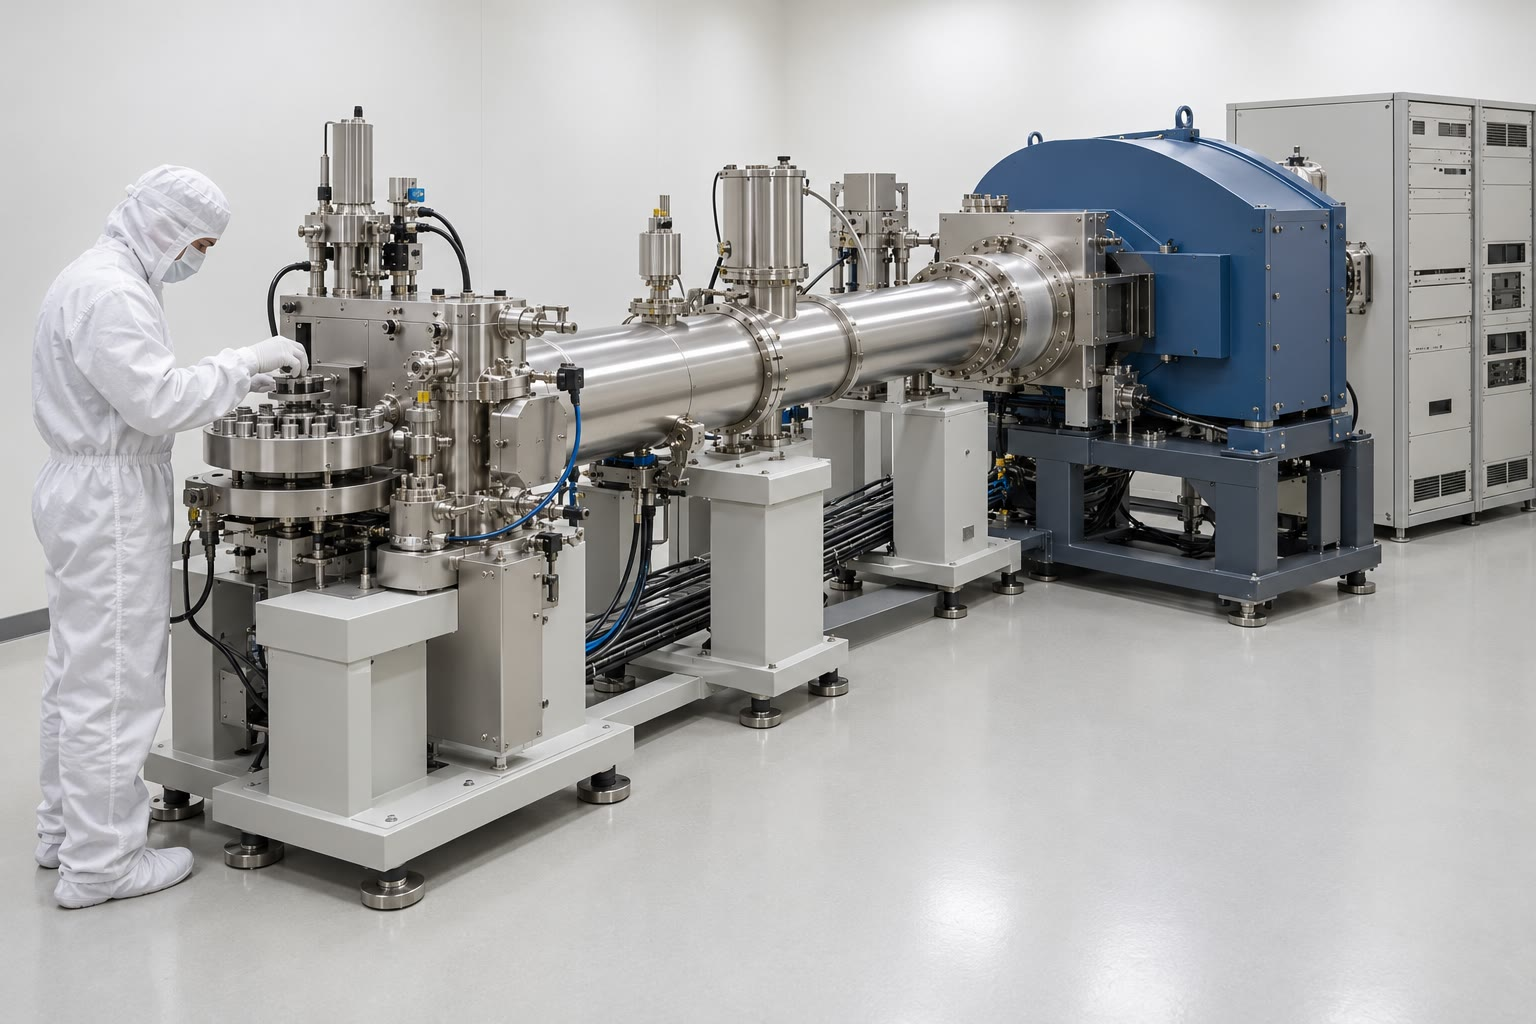
\includegraphics[width=\linewidth]{images/book5/ai/b3-mass-spec-lab.jpg}

{\scriptsize Un espectrómetro de masas en un laboratorio limpio: la torre de muestras a
la izquierda, el tubo de vuelo y el electroimán (ilustración
generada por IA).}
\end{minipage}
\end{inthelab}

\section{Datación argón--argón}\label{sec:b3:advanced-geochronology:arar}

El método potasio--argón del volumen de primer año mide el potasio y
el argón en dos alícuotas separadas de un mineral. El método argón--argón
mide solo argón, en una alícuota, como razones de isótopos. La muestra se
irradia con neutrones rápidos en el núcleo de un reactor nuclear, donde la
reacción $^{39}\mathrm{K}(n,p)^{39}\mathrm{Ar}$ convierte una fracción fija de su
potasio-39 en argón-39, un indicador del potasio. Un mineral de edad conocida, el
monitor, se irradia junto a ella.
% ledger: nmgrl:arar, amherst:arar

\begin{definition}[Datación argón--argón, factor J, espectro de edades, edad meseta]
\label{def:b3:advanced-geochronology:arar}
La \emph{datación $^{40}\mathrm{Ar}/^{39}\mathrm{Ar}$}\index{datación $^{40}\mathrm{Ar}/^{39}\mathrm{Ar}$}
data un mineral portador de potasio mediante la razón $R =
{}^{40}\mathrm{Ar}^*/{}^{39}\mathrm{Ar}_{\mathrm K}$ de su argón-40 radiogénico
al argón-39 formado a partir de su potasio por irradiación neutrónica. El
\emph{factor J}\index{factor J} de una irradiación es $J = (e^{\lambda
t_m} - 1)/R_m$, hallado a partir de un monitor de edad conocida $t_m$ y de la razón medida
$R_m$, siendo $\lambda$ la constante de desintegración total del potasio-40. Cuando la muestra
se desgasifica en etapas de temperatura creciente, su \emph{espectro
de edades}\index{espectro de edades} representa la edad de cada etapa frente a la
fracción acumulada de argón-39 liberado. Una \emph{edad
meseta}\index{edad meseta} es la media ponderada de las edades de etapas consecutivas que
concuerdan dentro de sus incertidumbres y liberan una gran parte del argón-39.
\end{definition}

\begin{theorem}[La edad argón--argón]\label{thm:b3:advanced-geochronology:arar}
Una muestra irradiada junto a un monitor tiene la edad
\[
t = \frac1\lambda\ln(1 + JR).
\]
\end{theorem}

\begin{proof}
El argón radiogénico es $^{40}\mathrm{Ar}^* = (\lambda_e/\lambda)\,
{}^{40}\mathrm{K}\,(e^{\lambda t} - 1)$, por la desintegración ramificada del
volumen de primer año. El argón-39 formado es $^{39}\mathrm{Ar}_{\mathrm K} =
{}^{39}\mathrm{K}\,\Phi$, donde $\Phi$ recoge la dosis neutrónica y la
sección eficaz de la reacción. Así, $R = (e^{\lambda t} - 1)/J$ con $J =
\lambda\,\Phi\,{}^{39}\mathrm{K}/(\lambda_e\,{}^{40}\mathrm{K})$. La razón
$^{40}\mathrm{K}/^{39}\mathrm{K}$ es la misma en todo el potasio, y $\Phi$ la
misma para dos muestras irradiadas lado a lado, así que $J$ es el mismo para la muestra
y el monitor; la edad y la razón del monitor lo determinan, e invertir $R$ da
$t$.
\end{proof}

Las constantes son las del método potasio--argón, $\lambda =
\qty{5.543e-10}{yr^{-1}}$. Un monitor habitual es una sanidina de una toba volcánica
datada en \qty{28.201}{\Ma}; una razón del monitor $R_m = 1.3129$ da $J =
0.01200$. El argón atmosférico, con $^{40}\mathrm{Ar}/^{36}\mathrm{Ar} = 295.5$,
se resta con el argón-36 medido en cada etapa, y el argón formado por
neutrones a partir del calcio y del propio potasio se corrige con sales
irradiadas en el mismo paquete.
% ledger: schaen20:monitors, amherst:constants, nmgrl:arar

El calentamiento por etapas es la gran fortaleza del método. La muestra se calienta en un horno
o con un láser en etapas de temperatura creciente, y cada etapa proporciona una edad.
Si el mineral permaneció cerrado desde que se enfrió, todas las etapas coinciden: el espectro es
plano. Si perdió argón de los bordes de sus granos, las primeras etapas, que
proceden de los bordes, son más jóvenes, y las edades suben en forma de escalera hacia una
meseta dada por los núcleos. Los criterios recomendados para una meseta son al
menos cinco etapas consecutivas que acumulan más de \qty{50}{\percent} del
argón-39, sin tendencia entre ellas; las etapas de baja temperatura de una escalera
suelen interpretarse como pérdida de argón radiogénico. El argón en exceso, atrapado a partir de un
fluido cuando el mineral creció, produce el efecto contrario: hace que algunas etapas sean demasiado viejas,
a menudo la primera y la última, en un espectro con forma de silla de montar. La suma de todas las
etapas, la edad del gas total, es lo que habría dado una edad potasio--argón: un
promedio que oculta la historia.
% ledger: schaen20:plateau, nmgrl:arar

\begin{omfigure}
\begin{tikzpicture}
\begin{groupplot}[group style={group size=2 by 1, horizontal sep=1.5cm},
  omrecord, height=0.38\linewidth, title style={font=\small},
  xlabel={$^{39}\mathrm{Ar}$ liberado acumulado (\unit{\percent})},
  tick label style={font=\scriptsize}, label style={font=\small}]
\nextgroupplot[title={(a) el espectro completo}, width=0.52\linewidth,
  ylabel={edad aparente (\unit{\Ma})}, xmin=0, xmax=100, ymin=130, ymax=320,
  xtick={0,20,40,60,80,100}, ytick={150,200,250,300}]
% computed in figdata/bachelor-3/arar_spectrum.py
\addplot[omDef, thick] table[x=cum, y=age] {figdata/out/bachelor-3-arar_spectrum-boxes.dat};
\node[font=\scriptsize, anchor=west] at (axis cs:12,180) {pérdida de argón};
\node[font=\scriptsize, anchor=north, red!70!black] at (axis cs:59,290) {meseta};
\nextgroupplot[title={(b) la meseta, ampliada}, width=0.44\linewidth,
  xmin=15, xmax=100, ymin=290, ymax=300, xtick={20,40,60,80,100},
  ytick={290,292,294,296,298,300}]
\addplot[name path=hi, draw=none, forget plot] table[x=cum, y=hi] {figdata/out/bachelor-3-arar_spectrum-boxes.dat};
\addplot[name path=lo, draw=none, forget plot] table[x=cum, y=lo] {figdata/out/bachelor-3-arar_spectrum-boxes.dat};
\addplot[omDef!25, forget plot] fill between[of=hi and lo];
\addplot[omDef, thick] table[x=cum, y=age] {figdata/out/bachelor-3-arar_spectrum-boxes.dat};
\draw[red!70!black, thick] (axis cs:18,296.1) -- (axis cs:100,296.1);
\node[font=\scriptsize, anchor=south, red!70!black] at (axis cs:59,290.3) {meseta \qty[separate-uncertainty=true]{296.1 \pm 0.8}{\Ma}};
\end{groupplot}
\end{tikzpicture}

\par\smallskip{\small El \omterm{def:b3:advanced-geochronology:arar}{espectro de edades} inventado de una biotita del granito de
la primera figura: cada etapa se dibuja a su edad, y su anchura es la fracción de
argón-39 que liberó. (a) Tres etapas de baja temperatura suben en escalera hasta una
meseta. (b) Las siete etapas de meseta, que concentran \qty{82}{\percent} del
argón-39, con sus intervalos de dos desviaciones típicas (sombreados) y la edad de
meseta (en rojo).}\label{fig:b3:advanced-geochronology:spectrum}
\end{omfigure}

\section{Edades modelo del neodimio}\label{sec:b3:advanced-geochronology:model-age}

Cuando un fundido se extrae del manto para formar corteza continental, el samario,
más compatible, queda en el residuo en mayor proporción que el neodimio: la nueva corteza tiene una
razón $^{147}\mathrm{Sm}/^{144}\mathrm{Nd}$ más baja que su fuente, de unos 0.13 en la mayoría de las
rocas corticales, frente a 0.1966 del reservorio condrítico. Su
$^{143}\mathrm{Nd}/^{144}\mathrm{Nd}$ crece entonces más lentamente. Una vez formada, una
roca cortical tiende a conservar su razón samario--neodimio, a través de la erosión,
la sedimentación e incluso la refusión, de modo que su neodimio recuerda cuándo salió del
manto.
% ledger: white08:model-age, white:chur

\begin{definition}[Edad modelo]\label{def:b3:advanced-geochronology:model-age}
La \emph{edad modelo}\index{edad modelo} de una roca en un sistema isotópico es el
tiempo en el que su razón, proyectada hacia atrás con la razón padre--hija actual,
iguala la de un reservorio modelo. Para el neodimio, $T_{\mathrm{CHUR}}$
emplea el reservorio condrítico uniforme y $T_{\mathrm{DM}}$ el manto
empobrecido.
\end{definition}

\begin{theorem}[Edad modelo]\label{thm:b3:advanced-geochronology:model-age}
Una muestra con razones actuales $I_s = {}^{143}\mathrm{Nd}/^{144}\mathrm{Nd}$ y
$R_s = {}^{147}\mathrm{Sm}/^{144}\mathrm{Nd}$, comparada con un reservorio de
razones actuales $I_m$ y $R_m$, tiene la \omterm{def:b3:advanced-geochronology:model-age}{edad modelo}
\[
T = \frac1\lambda\ln\left(1 + \frac{I_s - I_m}{R_s - R_m}\right),
\qquad \lambda = \lambda_{147}.
\]
\end{theorem}

\begin{proof}
Un sistema cerrado tenía, hace un tiempo $T$, la razón $I - R(e^{\lambda T} - 1)$: la
ecuación de la isócrona leída hacia atrás. Igualando esto para la muestra y el
reservorio da $I_s - I_m = (R_s - R_m)(e^{\lambda T} - 1)$.
\end{proof}

Con $\lambda_{147} = \qty{6.524e-12}{yr^{-1}}$, los reservorios son el
condrítico, 0.512638 y 0.1966 en la actualidad, y el manto empobrecido,
0.51315 en la actualidad, en torno a $\varepsilon_{\mathrm{Nd}} = +10$, valor que una
evolución cerrada a partir de valores condríticos desde hace \qty{4.55}{\Ga} da la razón
$^{147}\mathrm{Sm}/^{144}\mathrm{Nd} = 0.2137$. Un granito inventado con
$I_s = 0.511900$ y $R_s = 0.1100$ tiene $\varepsilon_{\mathrm{Nd}} = -14.4$
en la actualidad, $T_{\mathrm{CHUR}} = \qty{1.30}{\Ga}$ y $T_{\mathrm{DM}} =
\qty{1.84}{\Ga}$. La figura siguiente muestra ambas edades. La edad del manto empobrecido es la
mejor estimación, porque la corteza se extrae de un manto ya
empobrecido; es la edad media a la que el neodimio de la muestra salió del
manto, su edad de residencia cortical. Dos salvedades la limitan: la corteza no debe
haber cambiado su razón samario--neodimio desde entonces, y una roca formada por mezcla
de corteza antigua con fundidos de manto nuevo tiene una \omterm{def:b3:advanced-geochronology:model-age}{edad modelo} intermedia carente de significado.
% ledger: villa20:sm147, white:chur, white08:model-age

\begin{omfigure}
\begin{tikzpicture}
\begin{axis}[omrecord, width=0.72\linewidth, height=0.38\linewidth,
  xlabel={tiempo antes del presente (\unit{\Ga})}, ylabel={$\varepsilon_{\mathrm{Nd}}$},
  xmin=0, xmax=2.5, ymin=-17, ymax=13, x dir=reverse,
  xtick={0,0.5,1,1.5,2,2.5}, xticklabels={0,0.5,1,1.5,2,2.5},
  tick label style={font=\scriptsize}, label style={font=\small},
  legend style={font=\scriptsize, at={(0.5,1.03)}, anchor=south, legend columns=3, legend cell align=left}]
% computed in figdata/bachelor-3/model_ages.py
\addplot[omDef, thick] table[x=t, y=eps_dm] {figdata/out/bachelor-3-model_ages-evolution.dat};
\addlegendentry{manto empobrecido}
\addplot[black, thick, densely dashed] coordinates {(0,0) (2.5,0)};
\addlegendentry{CHUR}
\addplot[red!70!black, thick] table[x=t, y=eps_sample] {figdata/out/bachelor-3-model_ages-evolution.dat};
\addlegendentry{granito}
\draw[densely dotted] (axis cs:1.30,0) -- (axis cs:1.30,-17) node[above right, font=\scriptsize, rotate=90] {$T_{\mathrm{CHUR}}$};
\draw[densely dotted] (axis cs:1.84,5.4) -- (axis cs:1.84,-17) node[above right, font=\scriptsize, rotate=90] {$T_{\mathrm{DM}}$};
\end{axis}
\end{tikzpicture}

\par\smallskip{\small $\varepsilon_{\mathrm{Nd}}$ de un granito inventado proyectado
hacia atrás en el tiempo con su propia razón samario--neodimio (rojo). Alcanza el
reservorio condrítico en $T_{\mathrm{CHUR}} = \qty{1.30}{\Ga}$ y el manto empobrecido
(azul) en $T_{\mathrm{DM}} = \qty{1.84}{\Ga}$.}\label{fig:b3:advanced-geochronology:model-age}
\end{omfigure}

\section{Trazas de fisión y helio}\label{sec:b3:advanced-geochronology:low-t}

El uranio-238 también se desintegra, muy raramente, por fisión espontánea: el núcleo
se divide en dos fragmentos que salen despedidos y dejan un rastro de daño en el
cristal, de hasta \qty{9}{nm} de ancho y unos \qty{23}{\micro\metre} de largo en
apatito. Atacados con ácido, los rastros se hacen visibles al microscopio.
Se recuperan al calentarse el cristal, en un intervalo de unos 20 a \qty{350}{\celsius}
según el mineral; en el apatito se acortan en la zona de recocido parcial
de unos 60 a \qty{120}{\celsius}, y desaparecen por encima de ella.
% ledger: kohn24:ft, sueoka19:closure

\begin{definition}[Datación por trazas de fisión, recocido de trazas]\label{def:b3:advanced-geochronology:fission-track}
La \emph{datación por trazas de fisión}\index{datación por trazas de fisión} data un mineral por
la densidad de las trazas que deja en él la fisión espontánea del
uranio-238, comparada con su contenido en uranio. El \emph{recocido de
trazas}\index{recocido de trazas} es el acortamiento y la desaparición de las
trazas por reparación del cristal cuando se calienta.
\end{definition}

\begin{theorem}[La edad por trazas de fisión]\label{thm:b3:advanced-geochronology:fission-track}
Con $\lambda_f$ la constante de desintegración de la fisión espontánea y $\lambda =
\lambda_{238}$ la total, un cristal con $N_s$ fisiones espontáneas por unidad de
volumen y $N$ átomos de uranio-238 tiene la edad
\[
t = \frac1\lambda\ln\left(1 + \frac{\lambda}{\lambda_f}\,\frac{N_s}{N}\right).
\]
En el laboratorio, el uranio se mide induciendo la fisión del
uranio-235 con neutrones térmicos, y la edad pasa a ser
\[
t = \frac1\lambda\ln\left(1 + \lambda\,\zeta\,g\,\rho_d\,\frac{\rho_s}{\rho_i}\right),
\]
con $\rho_s$ y $\rho_i$ las densidades de trazas espontáneas e inducidas,
$\rho_d$ la densidad de trazas de un vidrio dosímetro, $g = 0.5$ un factor geométrico
y $\zeta$ una constante de calibración obtenida con patrones de edad conocida.
\end{theorem}

\begin{proof}
El uranio-238 se ha desintegrado $N(e^{\lambda t} - 1)$ veces, y la fracción
$\lambda_f/\lambda$ de estas desintegraciones fueron fisiones: $N_s =
(\lambda_f/\lambda)N(e^{\lambda t} - 1)$, expresión que se invierte en la primera forma.
Las densidades de trazas son proporcionales a $N_s$ y al número de fisiones inducidas,
$N\,\sigma\,\Phi/137.8$, donde $\sigma$ es la sección eficaz de fisión del
uranio-235 y $\Phi$ la fluencia neutrónica, a su vez
proporcional a $\rho_d$. La razón $\rho_s/\rho_i$ es entonces $N_s/N$ por
un producto de constantes, y $\lambda_f$, $\sigma$, $137.8$ y la eficiencia
del ataque químico y del recuento se agrupan con $g$ en $\zeta$.
\end{proof}

La constante de desintegración por fisión se conoce solo con una incertidumbre de unos \qty{10}{\percent},
entre \num{7.9e-17} y \qty{8.7e-17}{yr^{-1}}, por lo que la mayoría de
laboratorios prefieren la calibración con $\zeta$. Las longitudes de las trazas conservan
un registro de la trayectoria térmica. Una roca que se enfrió deprisa a través de la
zona de recocido parcial tiene trazas largas de longitud casi igual; una que
permaneció en ella tiene trazas más cortas de longitudes muy dispersas, y la
edad por trazas de fisión es entonces una edad mixta, no el momento de un paso por una
única temperatura.
% ledger: kohn24:ft

\begin{omfigure}
\begin{tikzpicture}[scale=0.85]
% (a) an etched apatite grain with tracks
\draw[thick, fill=omLithLime!15] (0,0) -- (3.2,0) -- (3.8,1.0) -- (3.2,2.0) -- (0,2.0) -- (-0.6,1.0) -- cycle;
\foreach \x/\y/\a in {0.4/0.5/30, 1.2/1.3/-20, 2.0/0.6/75, 2.6/1.4/10, 0.9/1.6/110, 1.7/0.9/150, 2.9/0.8/50}
  {\draw[very thick, black] (\x,\y) -- ++(\a:0.45);}
\node[font=\small] at (1.6,-0.4) {(a) trazas reveladas en apatito};
% (b) alpha ejection from a grain
\begin{scope}[xshift=6cm]
\draw[thick, fill=omLithLime!15] (0,0) rectangle (3.4,2.0);
\draw[dashed] (0.35,0.35) rectangle (3.05,1.65);
\fill[black] (0.2,1.0) circle (1.5pt) node[below right, font=\scriptsize] {U};
\draw[->, red!70!black, thick] (0.2,1.0) -- ++(160:0.7) node[left, font=\scriptsize] {He perdido};
\fill[black] (1.7,1.0) circle (1.5pt);
\draw[->, red!70!black, thick] (1.7,1.0) -- ++(40:0.5);
\node[font=\scriptsize, align=center] at (1.7,0.55) {He retenido};
\draw[<->] (3.05,1.8) -- (3.4,1.8) node[right, font=\scriptsize] {\qty{20}{\micro\metre}};
\node[font=\small] at (1.7,-0.4) {(b) expulsión alfa};
\end{scope}
\end{tikzpicture}

\par\smallskip{\small Esquema. (a) Trazas de fisión espontánea, reveladas por
ataque químico en un grano de apatito pulido, se cuentan por unidad de área. (b) Una partícula alfa
recorre unos \qty{20}{\micro\metre}: las emitidas dentro de esa
distancia de la superficie (fuera de la línea discontinua) pueden salir del grano, de modo que un
grano pequeño retiene menos de su helio.}\label{fig:b3:advanced-geochronology:low-t}
\end{omfigure}
% ledger: zeigler23:ejection

Cada desintegración alfa emite un núcleo de helio-4. El uranio, el torio y sus cadenas
acumulan helio en un cristal, que lo retiene solo cuando está frío.

\begin{definition}[Datación (U--Th)/He, zona de retención parcial]\label{def:b3:advanced-geochronology:uthhe}
La \emph{datación (U--Th)/He}\index{U--Th/He dating@datación (U--Th)/He} data un
mineral por el helio-4 acumulado a partir de las desintegraciones alfa del uranio, el torio
y sus descendientes, comparado con su contenido en uranio y torio. La \emph{zona de
retención parcial}\index{zona de retención parcial} es el intervalo de temperaturas en
el que el helio producido se retiene en parte y en parte se pierde por difusión.
\end{definition}

\begin{theorem}[Crecimiento del helio]\label{thm:b3:advanced-geochronology:helium}
Un cristal cerrado al helio durante un tiempo $t$ contiene
\[
\mathrm{He} = 8\,{}^{238}\mathrm U\,(e^{\lambda_{238}t} - 1)
+ 7\,{}^{235}\mathrm U\,(e^{\lambda_{235}t} - 1)
+ 6\,{}^{232}\mathrm{Th}\,(e^{\lambda_{232}t} - 1),
\]
en átomos, con los progenitores medidos en la actualidad; el samario-147 añade un término pequeño.
\end{theorem}

\begin{proof}
Cada cadena pierde su diferencia de masa en partículas alfa, cuatro unidades de masa cada una:
$(238 - 206)/4 = 8$, $(235 - 207)/4 = 7$, $(232 - 208)/4 = 6$, mientras que las
desintegraciones beta no cambian el número másico. Cada cadena está en equilibrio
secular, de modo que a cada desintegración del progenitor le sigue toda su cadena, y el
número de desintegraciones de cada progenitor es el de la ecuación de la edad.
\end{proof}

Para un cristal joven, $e^{\lambda t} - 1 \approx \lambda t$ y la edad se obtiene
con una sola división. Una partícula alfa recorre unos
\qty{20}{\micro\metre} antes de detenerse, así que un cristal pierde el helio producido
cerca de su superficie; la edad medida se divide entre la fracción retenida $F_T$,
que es menor en granos pequeños ($F_T = 0.70$ significa que se ha perdido
un \qty{30}{\percent}). El apatito cierra al helio hacia 50 a \qty{80}{\celsius}, el circón a
de 160 a \qty{200}{\celsius}: con las trazas de fisión del apatito, hacia 90 a
\qty{120}{\celsius}, los cronómetros de baja temperatura datan los últimos
kilómetros del ascenso de una roca hasta la superficie, tal como los empleó
el \cref{ch:b3:orogenic-wedges}.
% ledger: zeigler23:ejection, sueoka19:closure, iaea:isotopes

\section{Nucleidos cosmogénicos}\label{sec:b3:advanced-geochronology:cosmogenic}

Los rayos cósmicos que chocan contra la atmósfera producen lluvias de partículas
secundarias. Los neutrones rápidos que llegan al suelo rompen los núcleos de los minerales
de los primeros metros de roca, por espalación: el oxígeno del cuarzo se convierte en berilio-10, y el silicio
en aluminio-26. Los muones producen algunos nucleidos a mayor profundidad, y dominan por debajo de
unos \qty{3}{m}.
% ledger: zech04:exposure, portenga:method

\begin{definition}[Nucleido cosmogénico, edad de exposición, tasa de producción]
\label{def:b3:advanced-geochronology:cosmogenic}
Un \emph{nucleido cosmogénico}\index{nucleido cosmogénico} es un nucleido producido
en un mineral en la superficie o cerca de ella por las partículas secundarias de los rayos cósmicos. Su
\emph{tasa de producción}\index{tasa de producción (cosmogénico)} $P$ es el número
de átomos producidos por unidad de masa de mineral y por año. La \emph{edad de
exposición}\index{edad de exposición} de una superficie es el tiempo transcurrido desde que quedó
expuesta por primera vez a los rayos cósmicos, y se obtiene a partir de la concentración de un nucleido cosmogénico.
\end{definition}

La \omterm{def:b3:advanced-geochronology:cosmogenic}{tasa de producción} disminuye con la profundidad como $P_0e^{-\rho z/\Lambda}$, donde
la longitud de atenuación se toma como $\Lambda = \qty{160}{g.cm^{-2}}$, unos
\qty{60}{cm} de granito de densidad \qty{2.7}{g.cm^{-3}}. En la superficie aumenta con la altitud,
porque hay menos aire que proteja la roca, y con la latitud geomagnética,
porque el campo desvía menos partículas cerca de los
polos. Las tasas se dan para una referencia a nivel del mar y latitud alta, y se escalan
a cada lugar: una calibración da $P_0 = \qty{4.96}{\text{átomos}.g^{-1}.yr^{-1}}$
de berilio-10 en cuarzo para esa referencia. El berilio-10 tiene una vida media de
\qty{1.388}{Myr}, $\lambda = \qty{4.994e-7}{yr^{-1}}$.
% ledger: balco08:params, zech04:exposure, lugaro:slr-table

\begin{theorem}[Exposición con desintegración y erosión]\label{thm:b3:advanced-geochronology:exposure}
Una superficie que desciende a la tasa constante $\varepsilon$, expuesta durante un tiempo $t$
sin nucleidos heredados, conserva en su superficie la concentración
\[
N(t) = \frac{P_0}{\mu}\bigl(1 - e^{-\mu t}\bigr), \qquad
\mu = \lambda + \frac{\rho\varepsilon}{\Lambda}.
\]
Sin erosión, $N = (P_0/\lambda)(1 - e^{-\lambda t})$; tras un tiempo largo,
$N = P_0/\mu$, y sin desintegración esta es la fórmula $P_0\Lambda/(\rho\varepsilon)$
del volumen de primer año.
\end{theorem}

\begin{proof}
Sígase el grano que hoy está en la superficie. Hace un tiempo $s$ estaba a la
profundidad $\varepsilon s$, donde ganó átomos a la tasa $P_0e^{-\rho\varepsilon
s/\Lambda}$; de esos átomos queda hoy la fracción $e^{-\lambda s}$. Sumando
a lo largo de la exposición,
\[
N = \int_0^t P_0e^{-\rho\varepsilon s/\Lambda}e^{-\lambda s}\,\mathrm ds
= \frac{P_0}{\mu}\bigl(1 - e^{-\mu t}\bigr).
\]
Los límites se obtienen haciendo $\varepsilon = 0$, dejando que $t \to \infty$, y
después $\lambda = 0$.
\end{proof}

Sin erosión la concentración se satura en $P_0/\lambda$ tras unas pocas
semividas: una superficie alcanza el \qty{90}{\percent} de ese valor tras $\ln 10/\lambda
= \qty{4.6}{Myr}$, y a partir de ahí ya no puede datarse. Con erosión,
el estado estacionario se alcanza antes, tras unas pocas veces $1/\mu$, y su
concentración da $\varepsilon$; la tasa se promedia sobre el tiempo
$\Lambda/(\rho\varepsilon)$ que el grano tardó en ascender una
longitud de atenuación, unas pocas decenas de miles de años a las tasas de unas
pocas decenas de metros por millón de años. Los afloramientos de lecho rocoso se erosionan a unos pocos metros
a unas pocas decenas de metros por millón de años; las cuencas fluviales, medidas a partir de la
arena de sus ríos, más deprisa.
% ledger: portenga:rates, portenga:method

Dos nucleidos con vidas medias distintas datan el enterramiento. El berilio-10 y el
aluminio-26 se producen juntos en el cuarzo en una razón fija; cuando un grano
queda enterrado a gran profundidad en una cueva o bajo sedimento grueso, la producción se detiene,
y el aluminio-26, que se desintegra más deprisa, se rezaga: la razón entre ambos
varía con el tiempo y fecha el enterramiento.

\section{La estadística de una edad}\label{sec:b3:advanced-geochronology:statistics}

Una edad lleva asociada su incertidumbre, y un conjunto de edades plantea la
cuestión de si concuerdan. Sean $n$ medidas $x_i$ de una misma magnitud con
desviaciones típicas $\sigma_i$. Su media ponderada es $\bar x = \sum w_ix_i/W$, con
$w_i = 1/\sigma_i^2$ y $W = \sum w_i$, y su desviación típica es
$1/\sqrt W$.

\begin{definition}[Media de los cuadrados de las desviaciones ponderadas]\label{def:b3:advanced-geochronology:mswd}
La \emph{media de los cuadrados de las desviaciones ponderadas}\index{media de los cuadrados de las desviaciones ponderadas}
(MSWD) de $n$ medidas respecto a un modelo ajustado con $p$ parámetros
es
\[
\mathrm{MSWD} = \frac{1}{n - p}\sum_i \frac{(x_i - \hat x_i)^2}{\sigma_i^2},
\]
donde $\hat x_i$ es el valor del modelo: $p = 1$ para una media ponderada, $p = 2$ para
una recta como una isócrona o una \omterm{def:b3:advanced-geochronology:concordia}{discordia}.
\end{definition}

\begin{proposition}[El MSWD tiene esperanza igual a uno]\label{prop:b3:advanced-geochronology:mswd}
Si los $x_i$ son independientes y normales, con media $\mu$ y las desviaciones
típicas $\sigma_i$, el MSWD respecto a su media ponderada tiene esperanza 1.
\end{proposition}

\begin{proof}
Desarrollando $x_i - \mu = (x_i - \bar x) + (\bar x - \mu)$ y usando $\sum
w_i(x_i - \bar x) = 0$,
\[
\sum w_i(x_i - \mu)^2 = \sum w_i(x_i - \bar x)^2 + W(\bar x - \mu)^2.
\]
A la izquierda, cada término tiene esperanza 1, por lo que la suma tiene esperanza $n$. En
la derecha, $\bar x$ tiene varianza $1/W$, así que el último término tiene esperanza 1.
Por tanto, $\sum w_i(x_i - \bar x)^2$ tiene esperanza $n - 1$.
\end{proof}

El MSWD se dispersa alrededor de 1 de forma más amplia cuando hay pocos grados de libertad,
$f = n - p$: su límite superior al \qty{95}{\percent} es aproximadamente $1 +
2\sqrt{2/f}$, 2.63 para $f = 3$ y 2.15 para $f = 6$. Por encima del límite, las
medidas se dispersan más de lo que permiten sus incertidumbres: las muestras no tienen
todas la misma edad, o el sistema fue perturbado. Muy por debajo de 1, las
incertidumbres estaban sobreestimadas.
% ledger: schaen20:mswd

\begin{method}[Ajuste de una isócrona con errores en ambos ejes]\label{met:b3:advanced-geochronology:york}
Cuando ambas coordenadas llevan errores $\sigma_{x,i}$, $\sigma_{y,i}$, correlacionados
con el coeficiente $r_i$, como en los datos de uranio--plomo e isócronas:
\begin{enumerate}
\item partir de la pendiente $b$ de la recta de mínimos cuadrados ordinarios;
\item asignar a cada punto el peso $W_i = 1/(\sigma_{y,i}^2 + b^2\sigma_{x,i}^2 -
2br_i\sigma_{x,i}\sigma_{y,i})$, la inversa de la varianza de su distancia a la
recta medida a lo largo de $y$;
\item ajustar la recta ponderada con estos pesos, lo que da una nueva $b$, y
volver al paso 2 hasta que $b$ deje de cambiar;
\item calcular el MSWD con los pesos $W_i$ y $n - 2$ grados de libertad,
y la incertidumbre de la pendiente y de la ordenada en el origen a partir de los pesos finales.
\end{enumerate}
Con $\sigma_{x,i} = 0$ los pesos no dependen de $b$, y el método
se reduce a los mínimos cuadrados ponderados de $y$ sobre $x$ empleados en el problema.
\end{method}

La incertidumbre de una constante de desintegración es la misma para todas las edades de un sistema:
no interviene al comparar edades de un mismo sistema, pero debe sumarse
al comparar edades de dos sistemas. La constante de desintegración del samario-147, por
ejemplo, se conoce con una precisión de unos \qty{0.4}{\percent}; las del potasio-40,
de desintegración ramificada y lenta, limitan la precisión de las edades de argón.
% ledger: villa20:sm147, nmgrl:arar


\section{Ejercicios}

\begin{exercise}[$\star$]\label{exo:b3:advanced-geochronology:1}
Un circón tiene $^{206}\mathrm{Pb}^*/^{238}\mathrm{U} = 0.04500$ y
$^{207}\mathrm{Pb}^*/^{235}\mathrm{U} = 0.3300$. Calcúlense sus dos
edades uranio--plomo. ¿Es concordante? ¿A qué lado de la \omterm{def:b3:advanced-geochronology:concordia}{concordia} se
representa?
\end{exercise}
% ledger: amherst:constants

\begin{exercise}[$\star$]\label{exo:b3:advanced-geochronology:2}
Un monitor de \qty{28.201}{\Ma} da $R_m = 1.3129$. Calcúlese $J$ con $\lambda
= \qty{5.543e-10}{yr^{-1}}$, y después la edad de una muestra de la misma irradiación
con $R = 10.000$ (úsese $J = 0.01200$).
\end{exercise}
% ledger: schaen20:monitors

\begin{exercise}[$\star$]\label{exo:b3:advanced-geochronology:3}
Una lutita tiene $^{143}\mathrm{Nd}/^{144}\mathrm{Nd} = 0.51180$ y
$^{147}\mathrm{Sm}/^{144}\mathrm{Nd} = 0.1200$. Calcúlense sus $T_{\mathrm{CHUR}}$
y $T_{\mathrm{DM}}$ con los valores del capítulo.
\end{exercise}
% ledger: villa20:sm147, white:chur, white08:model-age

\begin{exercise}[$\star$]\label{exo:b3:advanced-geochronology:4}
Un bloque de cuarzo sobre una morrena en el sitio de referencia contiene \num{2.0e5}
átomos de berilio-10 por gramo. Suponiendo que no hay erosión ni herencia,
calcúlese su \omterm{def:b3:advanced-geochronology:cosmogenic}{edad de exposición} sin y después con desintegración, con $P_0 =
\qty{4.96}{\text{átomos}.g^{-1}.yr^{-1}}$.
\end{exercise}
% ledger: balco08:params, lugaro:slr-table

\begin{exercise}[$\star\star$]\label{exo:b3:advanced-geochronology:5}
Demuéstrese que cerca del origen la \omterm{def:b3:advanced-geochronology:concordia}{concordia} es una recta de pendiente
$\lambda_{238}/\lambda_{235}$, y calcúlese. Explíquese por qué la \omterm{def:b3:advanced-geochronology:concordia}{discordia} de
cristales que perdieron plomo solo muy recientemente pasa por el origen, y
qué mide la edad plomo--plomo de tales cristales.
\end{exercise}

\begin{exercise}[$\star\star$]\label{exo:b3:advanced-geochronology:6}
Cuatro edades de escalón de una meseta son $296.4 \pm 0.8$, $295.1 \pm 1.0$, $297.0 \pm
0.9$ y \qty[separate-uncertainty=true]{295.8 \pm 0.7}{\Ma} ($1\sigma$). Calcúlense su media ponderada,
su desviación típica y el MSWD. ¿Concuerdan?
\end{exercise}
% ledger: schaen20:mswd

\begin{exercise}[$\star\star$]\label{exo:b3:advanced-geochronology:7}
Un apatito tiene $\rho_s = \qty{1.20e6}{cm^{-2}}$ y $\rho_i =
\qty{2.40e6}{cm^{-2}}$, con $\rho_d = \qty{1.10e6}{cm^{-2}}$, $g = 0.5$ y una
calibración de laboratorio $\zeta = \qty{350}{yr.cm^2}$. Calcúlese su edad de trazas de fisión
¿Qué suceso data?
\end{exercise}
% ledger: kohn24:ft, sueoka19:closure

\begin{exercise}[$\star\star$]\label{exo:b3:advanced-geochronology:8}
Un apatito contiene \qty{20}{ppm} de uranio (\qty{99.2742}{\percent}
uranio-238, \qty{0.7204}{\percent} uranio-235 en átomos), \qty{40}{ppm}
torio-232 (semivida \qty{1.40e10}{yr}) y \qty{1.0}{nmol.g^{-1}} de helio.
Calcúlese su edad (U--Th)/He con la aproximación lineal, y después la edad
corregida por eyección alfa con $F_T = 0.75$.
\end{exercise}
% ledger: iaea:isotopes, zeigler23:ejection

\begin{exercise}[$\star\star$]\label{exo:b3:advanced-geochronology:9}
Para el berilio-10 en el emplazamiento de referencia, calcúlese la concentración de saturación
sin erosión y el tiempo necesario para alcanzar el \qty{90}{\percent} de ella. Calcúlese la
concentración estacionaria de una superficie que se erosiona a \qty{10}{m.Myr^{-1}} (granito,
\qty{2.7}{g.cm^{-3}}, $\Lambda = \qty{160}{g.cm^{-2}}$).
\end{exercise}
% ledger: balco08:params, zech04:exposure, lugaro:slr-table

\begin{exercise}[$\star\star\star$]\label{exo:b3:advanced-geochronology:10}
Se combinan dos medidas $x_1 \pm \sigma_1$ y $x_2 \pm \sigma_2$ de una misma
edad. Demuéstrese que su MSWD respecto a la media ponderada es
$(x_1 - x_2)^2/(\sigma_1^2 + \sigma_2^2)$, y demuéstrese directamente que su
esperanza es 1 cuando ambas miden la misma edad.
\end{exercise}

\begin{exercise}[$\star\star\star$]\label{exo:b3:advanced-geochronology:11}
Un circón de \qty{2700}{\Ma} perdió plomo a \qty{500}{\Ma} y hoy presenta
$^{206}\mathrm{Pb}^*/^{238}\mathrm{U} = 0.300$. ¿Qué fracción de su plomo
perdió? Calcúlese su $^{207}\mathrm{Pb}^*/^{235}\mathrm{U}$, sus dos edades uranio--plomo
y, por iteración, su edad plomo--plomo. ¿Cuál de las tres edades tiene
significado?
\end{exercise}

\begin{exercise}[$\star\star\star$]\label{exo:b3:advanced-geochronology:12}
Una superficie de lecho rocoso en el emplazamiento de referencia contiene \num{1.0e6} átomos de
berilio-10 por gramo. Calcúlese su \omterm{def:b3:advanced-geochronology:cosmogenic}{edad de exposición} suponiendo que no hay erosión, y después su
tasa de erosión suponiendo un estado estacionario. Demuéstrese que cada par $(t, \varepsilon)$
comprendido entre estos dos límites se ajusta a la medición, e indíquese qué segunda
medida los separaría.
\end{exercise}

\section{Problema: circones del granito de Varden}

\begin{problem}[{Problema de fin de semana --- la cristalización, el enfriamiento y
la exhumación de un granito inventado, interpretado con cuatro relojes}]\label{pb:b3:advanced-geochronology:1}
El granito de las colinas de Varden, región inventada de la serie, fue
exhumado ya en el Triásico, sepultado bajo la cobertera mesozoica y devuelto a la
superficie. Cinco de sus circones dan, con errores de una desviación típica en $y$
(tómese $x$ como exacto):
\begin{center}
\small
\begin{tabular}{|l|ccccc|}
\hline
circón & Z1 & Z2 & Z3 & Z4 & Z5 \\
\hline
$x = {}^{207}\mathrm{Pb}^*/^{235}\mathrm U$ & 0.3467 & 0.3260 & 0.3027 & 0.2793 & 0.2535 \\
$y = {}^{206}\mathrm{Pb}^*/^{238}\mathrm U$ & 0.04794 & 0.04505 & 0.04207 & 0.03892 & 0.03553 \\
$\sigma_y$ & 0.00010 & 0.00009 & 0.00008 & 0.00008 & 0.00007 \\
\hline
\end{tabular}
\end{center}
Utilícense las constantes del capítulo. Todos los análisis son datos de ejercicio.
% ledger: amherst:constants, schaen20:monitors, schaen20:plateau, schaen20:mswd, sueoka19:closure, balco08:params, lugaro:slr-table

\medskip\noindent\textbf{Parte I --- Los circones.}
\begin{enumerate}
\item ¿Son concordantes? Calcúlense las dos edades uranio--plomo de cada circón.
\item ¿Por qué disminuyen las edades de Z1 a Z5, con $t_{207} > t_{206}$ para
cada uno?
\item Calcúlense las coordenadas Tera--Wasserburg de Z1 y Z5.
\item Con los pesos $w_i = 1/\sigma_{y,i}^2$, calcúlense las medias ponderadas
$\bar x$ y $\bar y$, así como $S_{xx} = \sum w_i(x_i - \bar x)^2$.
\item Calcúlense la pendiente $b = \sum w_i(x_i - \bar x)(y_i - \bar y)/S_{xx}$ y
la ordenada en el origen $a$ de la \omterm{def:b3:advanced-geochronology:concordia}{discordia}.
\item Compárese $b$ con la pendiente de la \omterm{def:b3:advanced-geochronology:concordia}{concordia} cerca de \qty{310}{\Ma}. ¿Qué
anticipa esto?
\end{enumerate}

\medskip\noindent\textbf{Parte II --- Las intersecciones.}
\begin{enumerate}[resume]
\item Búsquese la \omterm{def:b3:advanced-geochronology:concordia}{intersección superior} por el método de Newton a partir de \qty{310}{\Ma}.
\item Búsquese la \omterm{def:b3:advanced-geochronology:concordia}{intersección inferior} a partir de \qty{100}{\Ma}.
\item Calcúlense los residuos ponderados y el MSWD. ¿Es aceptable el ajuste?
\item La desviación típica de la pendiente es $1/\sqrt{S_{xx}}$. Calcúlese.
\item Gírese la recta alrededor de $(\bar x, \bar y)$ hasta las pendientes $b \pm 2s_b$ y
recalcúlese la \omterm{def:b3:advanced-geochronology:concordia}{intersección superior} para cada una. ¿Cuál es la incertidumbre de la edad?
\item ¿Qué fracción de su plomo perdieron Z1 y Z5?
\end{enumerate}

\medskip\noindent\textbf{Parte III --- La biotita.} Una biotita del granito,
irradiada con un monitor de \qty{28.201}{\Ma} que da $R_m = 1.3129$, se
desgasifica en diez etapas:
\begin{center}
\small
\begin{tabular}{|l|cccccccccc|}
\hline
etapa & 1 & 2 & 3 & 4 & 5 & 6 & 7 & 8 & 9 & 10 \\
$^{39}\mathrm{Ar}$ (\unit{\percent}) & 4 & 6 & 8 & 12 & 14 & 15 & 14 & 12 & 9 & 6 \\
$R$ & 7.225 & 11.226 & 13.937 & 14.891 & 14.820 & 14.869 & 14.918 & 14.847 & 14.907 & 14.804 \\
edad (\unit{\Ma}) & & 228.0 & 279.0 & & 295.3 & 296.2 & 297.1 & 295.8 & 296.9 & \\
$\sigma$ (\unit{\Ma}) & 0.6 & 0.9 & 1.0 & 1.1 & 1.1 & 1.1 & 1.1 & 1.1 & 1.1 & 1.1 \\
\hline
\end{tabular}
\end{center}
\begin{enumerate}[resume]
\item Calcúlese $J$; redondéese a 0.01200.
\item Calcúlense las edades de las etapas 1, 4 y 10.
\item ¿Qué etapas forman una meseta según los criterios del capítulo?
\item Calcúlense la \omterm{def:b3:advanced-geochronology:arar}{edad meseta}, su desviación típica y su MSWD.
\item Calcúlense la razón y la edad del gas total. ¿Por qué es más joven que la meseta?
\item Suponiendo que el granito cristalizó a \qty{700}{\celsius} y que la
biotita cierra a \qty{375}{\celsius}, calcúlese la velocidad media de enfriamiento.
\item ¿Qué pudo ocurrir en la \omterm{def:b3:advanced-geochronology:concordia}{intersección inferior}? ¿Es el espectro de argón
consistente con ella?
\end{enumerate}

\medskip\noindent\textbf{Parte IV --- La exhumación.} Cuatro apatitos, muestreados
en una ladera de las colinas, dan edades (U--Th)/He de 43.1, 46.0, 49.2 y
\qty{52.0}{\Ma} a 310, 370, 430 y \qty{490}{m}. La cima del granito,
en una cresta suave de colina en un emplazamiento donde $P_0 = \qty{5.6}{\text{átomos}.g^{-1}.yr^{-1}}$,
contiene \num{1.64e5} átomos de berilio-10 por gramo de cuarzo.
\begin{enumerate}[resume]
\item Calcúlese la pendiente de la \omterm{def:b3:orogenic-wedges:age-elevation}{relación edad--altitud}, en metros por
millón de años.
\item Con una temperatura de cierre de \qty{65}{\celsius}, una superficie a
\qty{10}{\celsius} y una geoterma de \qty{30}{\celsius.km^{-1}}, ¿a qué profundidad
cerró el apatito más bajo? ¿Qué velocidad media de exhumación se deduce desde entonces?
\item Calcúlese la tasa de erosión actual a partir del berilio-10, suponiendo un
estado estacionario.
\item ¿Qué tasa da la fórmula del volumen de primer año, sin desintegración?
\item ¿Sobre qué intervalo de tiempo se promedia la tasa del berilio-10? Compárense las tres
tasas.
\item Establézcase la edad de cristalización del granito de Varden con su
incertidumbre.
\end{enumerate}
\end{problem}
